\documentclass{llncs}
\usepackage[T1]{fontenc}
\usepackage{algorithm}
%\usepackage{algorithmic}
\usepackage{algpseudocode}% http://ctan.org/pkg/algorithmicx


\usepackage{epsfig,endnotes,url,listings}
\usepackage{color}

\definecolor{dkgreen}{rgb}{0,0.6,0}
\definecolor{gray}{rgb}{0.5,0.5,0.5}
\definecolor{mauve}{rgb}{0.58,0,0.82}

\lstset{frame=tb,
  language=Java,
  aboveskip=3mm,
  belowskip=3mm,
  showstringspaces=false,
  columns=flexible,
  basicstyle={\small\ttfamily},
  numbers=none,
  numberstyle=\tiny\color{gray},
  keywordstyle=\color{blue},
  commentstyle=\color{dkgreen},
  stringstyle=\color{mauve},
  breaklines=true,
  breakatwhitespace=true,
  tabsize=3
}

\PassOptionsToPackage{usenames,dvipsnames}{xcolor}
\usepackage{wrapfig}

\usepackage{amssymb}
\usepackage{amsfonts}
\usepackage{amsmath} 
\usepackage{graphicx}
\usepackage{listings}
\usepackage{tikz}
\usepackage{pgf}
\usepackage{pgflibraryarrows}
\usepackage{pgffor}
\usepackage{pgflibrarysnakes}
\usepackage{xspace}

\usepackage{paralist}

%%Redefines lncs paragraph to have a bold title
%% \makeatletter
%% \renewcommand\paragraph{\@startsection{paragraph}{4}{\z@}%
%%                         {-12\p@ \@plus -4\p@ \@minus -4\p@}%
%%                         {-0.5em \@plus -0.22em \@minus -0.1em}%
%%                         {\normalfont\normalsize\bfseries}}
%% \makeatother

%% Save the class definition of \subparagraph
\let\llncssubparagraph\subparagraph
%% Provide a definition to \subparagraph to keep titlesec happy
\let\subparagraph\paragraph
%% Load titlesec
%\usepackage[compact]{titlesec}
%% Revert \subparagraph to the llncs definition
\let\subparagraph\llncssubparagraph


\newcommand{\jcupid}{\textsc{jCupid}\xspace}

\newcommand{\set}[1]{\left\{ #1 \right\}}
\newcommand{\Set}[1]{\big\{ #1 \big\}}
\newcommand{\seq}[1]{\langle #1 \rangle}
\newcommand{\Nat}{\mathbb N}
\newcommand{\Q}{\mathbb Q}
\newcommand{\R}{\mathbb R}
\newcommand{\Real}{\R}
\newcommand{\Int}{\mathbb Z}
\newcommand{\Rat}{\mathbb Q}
\newcommand{\Rplus}{\R_{\geq 0}}
\newcommand{\Zpos}{\Int_{\geq 0}}
\newcommand{\norm}[1]{\|#1\|}

\usepackage{wrapfig}



\usepackage[colorlinks=true]{hyperref}

\begin{document}

\title{\textsc{jCupid}: A dynamic analysis tool for detecting side channels in Java programs}
\author{
  Ian Martiny
  \and
  Eric Wustrow
  \and
  Pavol {\v C}ern\'y
  \and
  Ashutosh Trivedi
}
\institute{University of Colorado Boulder, USA \\
  \email{\{ian.martiny, ewust, pavol.cerny, ashutosh.trivedi\}@colorado.edu}}


\maketitle

\begin{abstract}
  Side-channel based vulnerabilities continue to plague modern security-critical
  applications.
  From leaking private-keys to exposing sensitive data, 
  protecting against these threats remains a difficult task for developers. 
  A common defense against side-channels is to write constant-time code.
  However, ensuring that a complex program has no data-dependent control flow
  can be a laborious challenge, and can on occasion introduce or enable new side
  channel vulnerabilities.
  We present \jcupid, a tool that aids developers in detecting and
  removing a particular class of side channels from their code.
  \jcupid dynamically tests Java programs for timing side channels by examining
  the sequence of bytecodes that are executed for multiple inputs of the same size.
  Our tool optimizes this process by first computing only hashes of bytecode sequences,
  so that comparing the full sequences becomes necessary only when a side-channel has been detected.
  Once two inputs are found that cause a different sequence of bytecodes to be
  executed, \jcupid can inform the developer of the offending line of source code
  responsible for the divergence.
  While our tool can naively fuzz an instrumented program, it can also be used
  in conjuction with a Concolic execution testing engine.
  We show that instrumenting programs for use with \jcupid is simple for
  developers, and that our tool can reveal timing side-channel vulnerabilities
  that are not immediately obvious from source code inspection.
\end{abstract}



\section{Introduction}
\label{sec:introduction}
%% Timing side channels are the bane of developers for security programs. The
%% prototypical example of flawed program with a timing side channel is a password
%% checker which verifies user input against a stored password one character at a
%% time and immediately reports results. This program leaks timing information back
%% to the user -- on an incorrect password, how many of the characters were correct
%% (more correct characters means longer execution time). 

%% Often side channels are much less obvious, and much more subtle. Even solutions
%% in order to prevent side channels can create their own side
%% channels~\cite{al2013lucky}. However these (sometimes subtle) side channels can
%% leak valuable information, sometimes even private key information. 

%% Thus it must fall to the developer to ensure that no extra information is leaked
%% when using their software. Our work here is to aid the developer in this
%% difficult and precise task. In order to do so we re-framed the problem of timing
%% information to \emph{work done}. Timing side channels are what we aim to
%% eliminate with this tool, however we approach this in an oblique manner. Our
%% motivation for this is that timing is \emph{hard}, especially over networks or
%% systems with noise. This may add some false sense of security to developers that
%% this difficulty is a defense, however as networks and systems get less noisy
%% this ``defense'' diminishes. 

%% We must endeavor to remove these side channels, ideally before the code is even
%% used in a release. To get around the difficulty of timing imbalances we have
%% focused in on Java programs, and the work that they do. In particular Java
%% programs run instructions: bytecodes. Our tool, jCupid, will attempt to
%% determine if there are a set of inputs which cause a program to execute
%% different bytecodes. Essentially asking the question: are there inputs which
%% make programs do different work? 


%\subsection{Related Work}
%% Attacks
Side-channel attacks are the class of attacks on cryptographic system that
attempt to gain information about a system by by exploiting involuntary
information leaks via physical properties---
such as temperature, electromagnetic leaks, memory footprints, and timing
delays---of the implementation rather than using brute force or exploiting
theoretical weakness of the algorithm.
Timing-based side-channel attacks are most common class of
side-channel attacks and are extremely powerful as physical isolation of the
server does not help and it is easier to observe the timing differentials than
temperature, memory, or electromagnetic leaks.  
Some notable examples of timing-based information leaks include \emph{padding oracle
attack}~\cite{Vau02}, \emph{Lucky-13 attack}~\cite{al2013lucky},  \emph{modular
exponentiator} employed in Diffie-Hellman, RSA, and DSS~\cite{kocher96}.

As an example of timing-based side-channel attack, consider modular
exponentiator used in Diffie-Hellman and RSA operations.
Here the system computes $R = y^x \mod n$ where $x$ is a secret key, $n$ is a
public information, and for an attacker it is easy to get hold of $y$.
In this attack the value $x$ of the secret key is fixed, and the attacker can
observe system response time for various combinations of $y$ and $n$.
A simple modular exponentiator algorithm is shown as Algorithm~\ref{alg:expo}.
Observe that in this algorithm a timing side-channel exists as depending upon
the value of the secret input, line $5$ may or may not be executed, and hence
algorithm will do different computation for different values of secret key, and
Kocher~\cite{kocher96} showed that it is sufficient to recover the secret key.
\begin{algorithm}[t]
Let $R = 1$\;
\For {$k = 0$ upto $w-1$}{
$R = R^2 \mod n$\;
\If {$x[k] = 1$}{
$R := (R \cdot y) \mod n$\;
}
}
\Return $R$\;
\caption{A Simple Modular Exponentiator Algorithm}
\label{alg:expo}
\end{algorithm}

A na\"ive remedy to timing-based information leaks in software-implemented
systems is to make the software run in fixed time for all possible inputs by
introducing timers to delay the observable outputs. 
However, it is quite difficult to ensure in practice, and even in the presence
of such timers CPU usage may also leak same information.
Molnar et al.~\cite{Molnar05} proposed to model side-channels with
so-called \emph{transcript security model} where the sequence of certain
observable variable (transcripts) is leaked to the attacker.
Under this setting a program is secure if the adversary learns nothing about the
secret value even after given access to the side-channel transcripts.
Among others, program counters and opcodes, have been proposed as an appropriate
notion of observable variables for transcripts.
Molnar et al.~\cite{Molnar05} present a run-time profiler for C programs to
detect side-channels by reporting pair of inputs that differ in program-counter
transcripts.  
In this paper we propose a similar runtime profiler to test whether a given
Java program is transcript secure where transcripts are Java Bytecode
instructions for inputs of same size.
Our framework, with some efforts, can be extended to more general notions of
transcripts.

Fuzz testing techniques~\cite{God12} are scalable and effective techniques for finding security
vulnerability in software.
Godefroid, Levin, and Molnar~\cite{God12} popularized the distinction between
blackbox and whitebox fuzz-testing techniques.
In blackbox fuzz-testing approach well-formed inputs are randomly modified,
while conforming to a template given as formal grammar and probabilistic
weights, to generate other potentially interesting inputs.  
Some popular tools for blackbox fuzzing include Peach 
(\url{http://www.peachfuzzer.com/}) and Autodafe
(\url{http://autodafe.sourceforge.net/}).
In contrast, whitebox fuzzing techniques---introduced by Godefroid et
al.~\cite{God12,GKS05}---exploit symbolic execution and dynamic test-case generation
to systematically generate test-cases to exercise different control-paths by
negating conditions exercised by previous test-cases.
CUTE and jCUTE~\cite{Sen2006} are popular whitebox fuzzing tools for C and Java
programs. 
The run-time profiling framework that we propose in this paper can be
effectively combined with both blackbox and whitebox fuzz testing techniques to
automate generation of interesting inputs.

An issue related to testing and verification of transcript security of a program
is the automatic synthesis of transcript-secure programs from un-secure ones.
Eldib and Wang~\cite{EW14} proposed a synthesis method (and tool SC Masker)
based on LLVM compiler and Yices SMT solver to produce a perfectly-masked
program such that resulting program is such that all the observable outputs are
statistically independent from the input data. 
Prouff and Rivain~\cite{PR13} outline a formal security proof for masked
implementations of block ciphers.      

For a background on formal quantitative information flow we refer the reader to
an excellent introductory article by Smith~\cite{smith09} and references therein.
Static and dynamic information flow techniques~\cite{SR10,Den76} have concentrated
mainly upon explicit and implicit information flow from secret variables to
outputs or observable variables.
However, side-channel information is often not explicitly present in the text
(source code or bytecode) of the program.
A key challenge under this assumption is to make this timing side-channel
explicit by learning timing function of various program units in the software
and use them to either statically analyze the software for side-channel freedom,
or use run-time profilers to execute inputs of similar size such that the
observable input differs.
Our tool is an attempt in this direction.

%% \subsection{Old Part}
%% The idea monitoring executed bytecodes is not dissimilar to that of finding all
%% of the paths through a program. This led us to many concolic testers and input
%% fuzzers.  

%% In particular jFuzz~\cite{jayaraman2009jfuzz}, a concolic whitebox input fuzzer,
%% built on the NASA Java PathFinder. The goal of jFuzz is to start from a given
%% seed and using this find inputs which lead down all possible paths of a given
%% program. As mentioned this goal is not completely perpendicular to our own, and
%% finding which inputs lead down unique paths is valuable information. This
%% project however was difficult to get running, as it requires Java 1.5, and
%% seemingly does not work with Java 1.8. 

%% Additionally another concolic tester, jCute~\cite{conf/cav/SenA06} allowed us to
%% use more recent versions of Java. While jCute was a promising tool we found that
%% that for some of our test programs jCute did not recognize various paths in our
%% program. 





\section{\textsc{jCupid}}
\label{sec:jcupid}

\jcupid consists of a python script that wraps a modified version of OpenJDK.
Our python wrapper runs a specified program multiple times through our modified
OpenJDK, looking for two inputs that provide different bytecodes executed. We
have several optimizations to make this performant, which we detail in this
section.

\subsection{OpenJDK}
\label{sec:OpenJDK}

While OpenJDK already provides a feature for printing out executed bytecodes in
debug mode (with the \texttt{-XX:+TraceBytecodes} flag), we found that using
this feature for our tool proved to be significantly too slow. In addition,
this prints out a large number of bytecodes used in the initialization and
startup of the program. For example, a simple ``Hello World'' program executes
1.18 million bytecodes, while only 6,054 of those bytecodes are actually within
the \texttt{main} method. In addition, even just running this simple program
takes 8.6 seconds to execute using the \texttt{-XX:+TraceBytecodes} flag.
% 1,179,829 bytecodes executed total

Rather than using the \texttt{-XX:+TraceBytecodes} option and inspecting the
output to determine the bytecodes executed for a given program run, we modified
OpenJDK and added a new feature that hashed the bytecodes as they were executed,
and then printed out the final hash after the program terminated. As we do not
need a cryptographic hash for this purpose, we used the lightweight djb2 hash
function~\cite{djb2Hash}.

In addition to hashing, we also added a feature to allow the user
to specify the class and method for when this hashing should start and end, so
that extraneous bytecodes executed during program initialization can be ignored.
This feature is also available during the use of the
\texttt{-XX:+TraceBytecodes} option, limiting the bytecodes that are printed to
the method specified by the user. With these two features, a simple ``Hello
World'' program can be run in about 0.8 seconds, ten times faster than using
the \texttt{-XX:+TraceBytecodes} flag.

With this feature, our python wrapper can simply generate inputs, and receive
the hash of the bytecodes executed in the relevant class/method for that input.
Once the python script determines two inputs that produce different hashes, it
knows the execution has diverged. The script then follows up by using the
slower \texttt{-XX:+TraceBytecodes} flag on both instances of the program, and
compares their outputs to detect the deviation. 

%To help in this we modified OpenJDK to allow for new flags: \texttt{-hashClass}, \texttt{-hashMethod}, \texttt{-traceClass}, and \texttt{-traceMethod}. Each takes an argument, a class name or method name respectively. The \texttt{-hashClass} and \texttt{-hashMethod} flags are used together as are the trace variants. Their arguments dictate the class and method that we are interested in. For example in Listing~\ref{lst:ex} we would be interested in the class \texttt{SumRandomBytes} and the method \texttt{main}. Though in general the user could specify any class/method in their program. 


\subsection{Inputs}

jCupid chooses inputs automatically, attempting to find two inputs that produce
different execution traces. \jcupid can generate inputs in two ways. First, it
can generate a random string input, such as the ones used for our sample
programs. Second, \jcupid can work with jCute, a concolic execution testing tool
for Java programs that can statically determine a set of inputs to maximize code
coverage during execution. Unfortunately, we found that jCute was unable to
produce even obvious inputs for some of our toy programs, so we simply used our
former method, generating random strings of the same length as inputs to our
programs.


\subsection{Informing the Developer}

Once we find two inputs that produce different execution traces, \jcupid will
use the \texttt{-XX:+TraceBytecodes} flag, and find the differing bytecodes. It
then uses the \texttt{javap} utility in combination with the bytecode output to
determine what line of source code is responsible for producing those bytecodes.
Thus, we can inform the developer of the line in their code that is responsible
for this potential side channel, as well as the two inputs to their program that
cause it to diverge there.


%\begin{figure}[t]
%  \begin{center}
%    \begin{lstlisting}[language=make,caption={Example output from OpenJDK with trace flags set},label={lst:sample}]
%static void SumRandomBytes.main(jobject)
%     0  new 2 <java/util/Scanner>
%
%virtual jobject java.lang.ClassLoader.loadClass(jobject)
%     0  fast_aload_0
%     1  aload_1
%     2  iconst_0
%     3  invokevirtual 41 <java/lang/ClassLoader.loadClass(
%     Ljava/lang/String;Z)Ljava/lang/Class;> 
%    \end{lstlisting}
%  \end{center}
%\end{figure}

%\begin{figure}[h]
%  \begin{center}
%    \begin{lstlisting}[language=make,caption={Example output from \texttt{javap}},label={lst:lines}]
%public static void main(java.lang.String[]);
%    LineNumberTable:
%      line 31: 0
%      line 33: 11
%      line 35: 16
%      line 37: 21
%      line 40: 26
%      line 51: 32
%      line 42: 35
%      line 44: 37
%      line 45: 45
%      line 51: 49
%      line 47: 52
%      line 49: 54
%      line 50: 62
%      line 56: 66
%      line 57: 73
%      line 63: 81
%      line 59: 84
%      line 61: 86
%      line 62: 94
%      line 65: 98
%    \end{lstlisting}
%  \end{center}
%\end{figure}
%

%\subsection{OpenJDK Details}
%OpenJDK~\cite{OpenJDK} provided us with the ability to look at executed
%bytecodes. The key word here being \emph{executed} bytecodes, there are numerous
%static analyzers that allow the user to examine the bytecode information of
%their code~\cite{vallee1999soot}. However a bytecode (or timing) difference can
%occur in a library call and as such we need to dynamically analyze bytecodes
%that are executed on each run. The OpenJDK project is an open-source version of
%Oracle's JDK. This was key for jCupid due to certain flags for the JDK
%(\texttt{-XX:+TraceBytecodes}) are only allowed in develop versions of the JDK,
%compiled with a debug flag. The release version of the JDK does not allow the
%use of this flag, however compiling OpenJDK with the debug flag allowed us
%access to dynamically executed bytecodes. Listing~\ref{lst:ex} shows an example
%of code in which bytecode differences will occur not in the source code but in a
%library call. The \texttt{SumRandomBytes} program will read a string from the
%user and then sum the bytes of the characters. This sum gives the number of
%bytes to read from a file which are then hashed. The hash function will do
%different amounts of work based on the given input string. 
%
%The above projects are great tools, but do not solve the problem at hand, which
%is to pinpoint which bytecode, or line of code causes a program do different
%work for different inputs. This is what jCupid attempts to help solve with the
%aid, or incite of the above projects. 
%
%\begin{figure}[t]
%  \begin{center}
%    \begin{lstlisting}[caption={Example of code with bytecode difference in
%    Library call},label={lst:ex},language=Java] 
%public class SumRandomBytes
%{
%  public static void main(String [] args)
%  {
%    Scanner sc = new Scanner(System.in);
%    String s = sc.nextLine();
%
%    int sumOfBytes = sumString(s);
%    byte [] data = new byte[sumOfBytes];
%
%    data = readBytes(sumOfBytes);
%
%    MessageDigest md = MessageDigest.getInstance("SHA-1");
%    md.digest(data);
%  }
%}
%    \end{lstlisting}
%  \end{center}
%\end{figure}


\section{Evaluation}
\label{sec:evaluation}
We evaluated \jcupid using a set of simple programs that commonly contain timing
side channels in their implementations.

\begin{itemize}
\item \textbf{Password checking.}
The na\"{\i}ve method of checking whether a provided password is correct is to iterate
over the provided input, comparing each character to its expected value, and
returning failure on the first discovered difference. This results in a side
channel that leaks the number of characters that an attacker has guessed
correctly, allowing them to perform an adaptive attack. The attacker can guess
each character independently, and only move on to the next character when they
have found the correct character in the current position. While we call this a
password checking test case, this pattern also occurs in any string comparison
that should be done in constant time, such as when checking if CSRF or
authentication tokens are valid.

%\textbf{Lucky-13 attack}
%We implemented a toy Java version of the padding and MAC check employed in TLS
%decryption. Our implementation was vulnerable to the Lucky 13 attack, where
%an attacker modifies ciphertext, and can distinguish between the corresponding
%plaintext having valid padding or not. This capability allows an attacker to
%perform a Vaudenay attack and iteratively leak the plaintext.
\item 
\textbf{Modular Exponentiation.}
We implemented the straightforward method for modular exponentiation shown in
Algorithm~\ref{alg:expo}. This algorithm has a side-channel dependent on the
(private) exponent input. To compare against a side-channel-free version,
we also implemented a variant on the Montgomery Ladder
technique for modular exponentiation. However, we had to use algebraic tricks to
replace the branches that are present in the algorithm. Our updated version has no
data-dependent branches, and relies only on multiplication, addition,
subtraction, and modulus operations.

\item
\textbf{SumBytes.}
We created a program that reads a single byte to determine a length, then reads
that many bytes and hashes them. Here, we are mimicking a simple serialized
network protocol with a length encoded at the beginning of the message. The side
channel present in this code is subtle: there are no if statements or obvious
branches in the code. Rather, the number of bytes read determines the number of
compression function iterations occur internal to our hash function.
\item 
\textbf{Multiplexer.}
Finally, we implemented a selection function that takes three inputs: a, b, and
a selector. If the selector is true, our function returns the first input,
otherwise it returns the second input. This is easily accomplished by an if
statement, however, such an implementation may leak information due to instruction cache timing or
memory accesses.
\end{itemize}
%\bigskip

For each of these programs, we allowed them to take a single input as a string
on standard input. Then, we allowed \jcupid to fuzz these programs with random
inputs, and look for potential differences in the bytecodes executed. In each
example, we found the intended side-channel, and \jcupid was able to correctly
determine the line of code responsible.

We then corrected the problems identified by \jcupid, and reran our tool to
verify we had removed the offending side-channels. To our surprise, \jcupid
identified additional problems in some of our ``corrected'' programs. For example, in
the password checking program, we used a temporary value, and updated it at each
iteration with \texttt{good \&= (input[i] == expected[i])}. However, this resulted in
a side-channel when computing the \texttt{==} operator, as Java implemented this as a
branch in the bytecode. We fixed this by switching to using exclusive-or to
compare the values, and \jcupid did not detect any additional side-channels. This
further illustrates the difficulty of removing all potential side-channels from
code: even seemingly branch-free programs, written with the intention of not
having side-channels, can contain them.


As \jcupid is a dynamic analysis tool, it must run many instances of the program
in order to find side-channel behavior. We evaluated \jcupid's overhead by
measuring how quickly it can run basic Java programs, and compared it to
running those same programs outside of the \jcupid environment. Particularly for
a developer dynamic analysis tool that inspects individual bytecodes, our
results are encouraging: per run, \jcupid only adds on average approximately 2x
overhead. This could allow even rare side-channels to be detected with
na\"{\i}ve fuzzing of nightly builds over unit tests.

\paragraph{Timing experimentation.}
In order to test the efficiency of \jcupid, we ran a number of experiments to
determine how much overhead \jcupid has, and where the overhead comes from.
With the above test programs, we ran each program 10 times with an unmodified
OpenJDK. Then, we ran each program using our tool with 10 iterations. Over all
of the runs, we found that stock OpenJDK took on average 2.6 seconds per
iteration, while \jcupid took on average 5.3 seconds per iteration. However, this
is obviously variable based on the input program: for longer running and more
computationally-expensive programs, we observe that \jcupid's overhead is lower.

To determine which components of \jcupid are responsible for its overhead, we
removed individual components and reran our programs. We ran our Python tool in
a way that it called a normal OpenJDK rather than our modified (debug) one, and
found that it took on average 3.6 seconds per run. We then ran our tool using a
modified version of OpenJDK that did not use hashing, and found it takes 4.8
seconds. Thus, we estimate that our Python tool adds about half of the overhead
of \jcupid,
with the remainder coming mainly from the debug version of OpenJDK, and a small
contribution from the fast hash function itself.

%with the inputs. Then we ran the programs with a modified version of our tool 
%which simply calls OpenJDK, with no flags -- this allows us to test how much 
%overhead the tool itself has. Finally we run the tool on a modified OpenJDK such
%that the hash function does no work (meaning nothing will be flagged) -- this 
%tells us how much time our hash function is taking. Each of the above tests are 
%run 5 times.
%
%Averaging the time results across the different programs provides the following
%results: just calling OpenJDK takes around 2.6 seconds, \jcupid averages 5.3 seconds
%per call to OpenJDK. This is an overhead of 2.7 seconds. The following two results
%will help us determine where this overhead comes from. With the modified \jcupid tool
%that just calls OpenJDK with no flags takes 3.6 seconds, and finally calling \jcupid
%that calls a modified OpenJDK that does not do hashing takes 4.8 seconds.
%
%The above results tell us that of the 2.7 seconds of overhead 1.0 seconds of overhead
%come from the tool itself, and 1.2 second of overhead comes from the flags that
%we use in \jcupid. Thus the remaining 0.5 seconds of overhead come from the hash
%function itself.


\section{Future Work}
\label{sec:future}
There are many avenues for future work on this project. In particular, 
we plan to use, and potentially adapt, a concolic tester, in order to
cover all control-flow paths in a program. Our initial experiments
show that jCute~\cite{Sen2006} was much faster
at finding inputs of interest than the random fuzzer that we
implemented (as would be expected). We would need to adapt the
concolic tester as not only would we want this tester to
be able to find all paths, but also find paths that are reachable under
given constraints, such as input length. 

Another interesting avenue is to refine this tool to examine the types
of differences we see in bytecode execution. In particular, it may be
that in certain programs, there are no timing
differences, but the sequences of executed bytecodes are different. As
the goal of the tool is to find timing side channels, this would lead to
false positives. Thus it would be interesting to 
collect bytecodes into equivalence classes by time and allowing
differences in execution within these classes. 

Finally, this project was written for Java programs, it would be a noteworthy
extension to continue this project in C to let a greater audience
access the tool. 


\section{Conclusion}
\label{sec:conclusion}
Timing side-channels are a great concern when developing 
secure programs. With \jcupid, we hope to aid developers in writing
code that is timing side-channel free. In order to find the side
channels, \jcupid 
tracks the sequence of bytecodes that are executed for multiple inputs
of the same size. Once two inputs are found that cause a different
sequence of bytecodes to be executed, \jcupid can inform the developer
of the line that caused the
divergence. We show that in this way \jcupid can detect side channel
bugs using a series of case studies (and we show that \jcupid does not
detect bugs in the corrected versions).

This tool is intended to be used by developers to test very
specific aspects of their code. Running \jcupid on even moderately sized
projects, say an authentication server, will most
certainly find different bytecodes executed based on input (even of
the same length). \jcupid is intended as a more precise tool. Instead of 
analyzing the whole server, the tool is
intended to analyze whether the modular exponentiation function
executes different bytecodes for inputs of the same size (and thus for
instance reveals information about bits in the secret key). 



\bibliographystyle{plain}
\bibliography{papers}

\newpage
\appendix
% Appendix 

\section{Appendix: \jcupid demo}

Presenter (P): jCupid is a python script wrapped around a modified version of OpenJDK. jCupid's goal
is to assist developers in fixing timing vulnerabilities in their code. The user would provide a sample
Java program and specific method to test for timing vulnerabilities. jCupid would then choose various
inputs to give to the program and examine the bytecodes that are executed.

As opposed to timing the the run of the program jCupid actually analyses the bytecodes that the program
executes, the idea being that a given program should do exactly the same instructions for all input.

jCupid achieves this by using some functionality of the debug version of the OpenJDK as well as some
modifications that were made. Namely jCupid will provide OpenJDK with the name of the class and method
the user is interested in, then from the time that the method begins execution until it returns OpenJDK
will run a quick hash of all of the bytecodes that are executed. This provides a quick way of determining
whether the inputs are doing different work, if they produce different hashes, then jCupid will dive 
in more in depth into those executions, but inputs that lead to the same hash do not need extra time
spent on them. As mentioned after different hashes are produced by inputs those inputs are provided
to the program again with different flags for OpenJDK that will provide a list of all the bytecodes 
executed (in order). Then jCupid will then compare those outputs to find the bytecode that is different
and finally work to find the line of source code that presented this difference.

When calling jCupid the user must provide certain information namely: the filename of the java program,
the name of the class and method that the user is interested in testing, the length of inputs to provide
to the program and the maximum number of iterations to run. Thus a potential call to jCupid would look
as such:

\begin{center}
  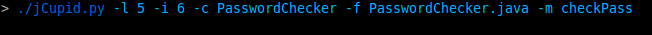
\includegraphics[width=\linewidth]{jCupidCall}
\end{center}

Which tells jCupid that it should use at most 6 random strings of length 5 to run the file PasswordChecker.java
and to examine the method checkPass in the class PasswordChecker. A quick look at that function tells us how
it will check passwords:

\begin{center}
  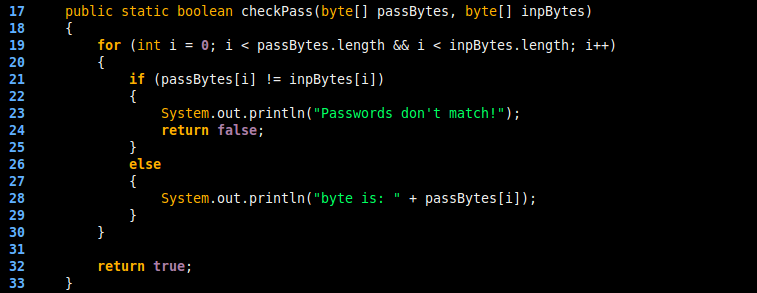
\includegraphics[width=\linewidth]{PasswordChecker}
\end{center}

As we can see this is the simple way of checking passwords, one character at a time and immediately reporting
any failures. This definitely would lead to a timing vulnerability. For reference the password is 
``mySecretPassword'', so we should see some different bytecodes executed between inputs that start with `m'
vs ones that don't. Lets see how jCupid handles this:

\begin{center}
  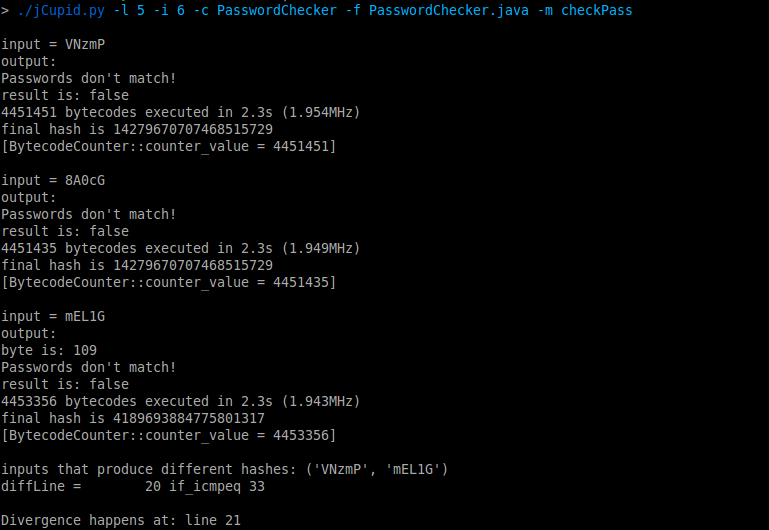
\includegraphics[width=\linewidth]{jCupidRun1}
\end{center}

Here we see that jCupid tells us what it is inputting. The first input is ``VNzmP'', the first character
isn't `m' so we know it will fail immediately. jCupid then shows the output from the program and some
diagnostic output including how many bytecodes were executed and the result of the hash. The second input
is ``8A0cG'' which again should fail immediately and we can see it has the same hash and moves on to the
next input. The third input is ``mEL1G'', this input should lead us down a different path since the first
character matches the first character of our password. Indeed we can see that the hash for this input is
different. This prompts jCupid to now look for the offending bytecode and trace this back to a line in 
the source code, in this case it tells us line 21 is the offending line, which we can see is the line of
the \texttt{if} statement.

The now informed developer can recognize their mistake and fix this code! One common way of ``correctly''
checking passwords is to always loop through the provided password and simply update a counter by and-ing
whether each character matches the correct password. This implementation can be seen here:

\begin{center}
  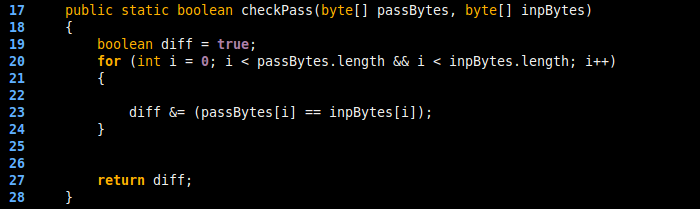
\includegraphics[width=\linewidth]{PasswordCheckerFix1}
\end{center}

This fix looks good! We always examine the full length of the input and are simply updating a variable
with the exact same line of code no matter what. Lets see what jCupid says:

\begin{center}
  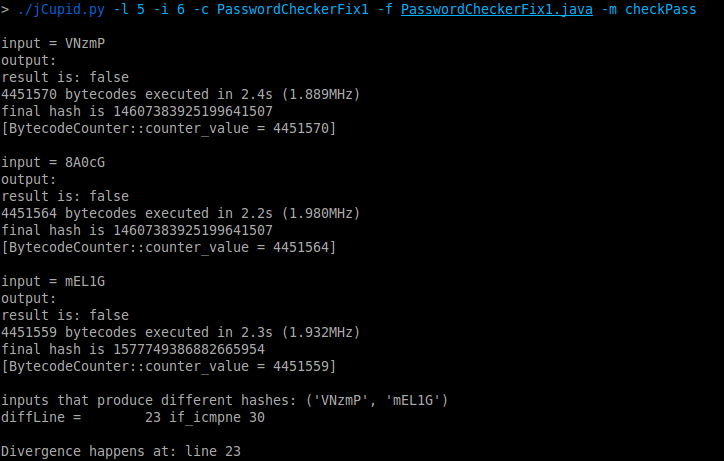
\includegraphics[width=\linewidth]{jCupidRun2}
\end{center}

Running the same inputs through again we see that indeed the two first inputs do the same work, as expected,
but suprisingly we still get different bytecodes executed with this fixed solution. After much investigation
it appears that a peculiarity of Java turns the $==$ into an if statement! Luckily we ran the code through
jCupid again. After some clever thinking we may realize that we need to do this checking without actually
comparing the characters, but we can do a computation on them. Specifically we can xor each character to
determine if they are the same, and then keep a running \texttt{or} to keep track of any differences showing
up. So the code now looks like:

\begin{center}
  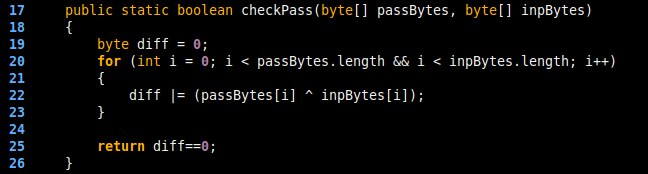
\includegraphics[width=\linewidth]{PasswordCheckerFix2}
\end{center}

Now there are no decisions being made at all in the code, just a computation being done, and the same 
computation. Lets see if jCupid agrees with us:

\begin{center}
  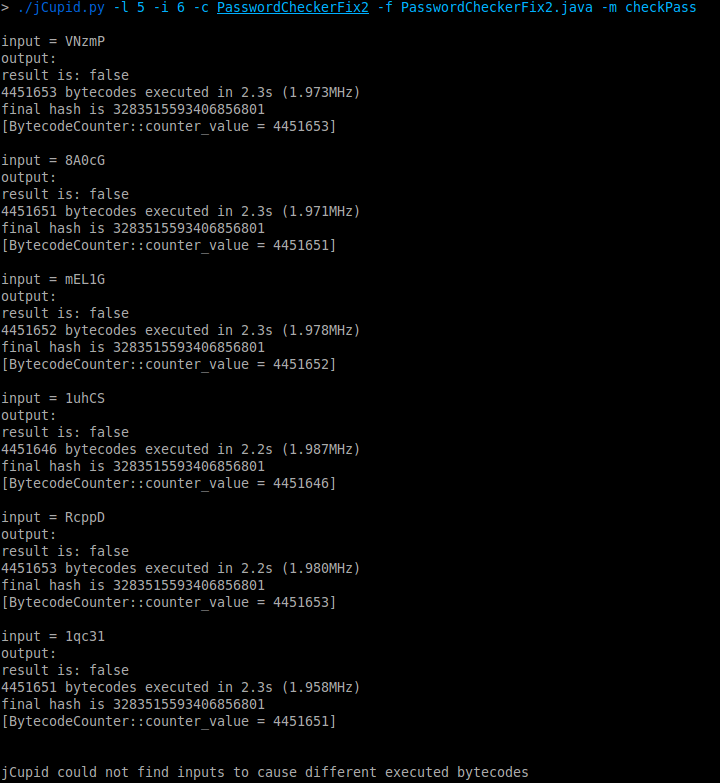
\includegraphics[width=\linewidth]{jCupidRun3}
\end{center}

Indeed we can see that jCupid found no difference between any of the inputs, regardless of whether they 
began the same as the password. Of course we would want to run significantly more trials on numerous 
length inputs in order to be more confident, but we can see that we have fixed our problem of matching
letters causing different instructions to be executed. Even though the first solution we had seemed like
it was exactly what we wanted, Java's compiler changes the code in subtle ways that can add side-channels.

It is worth noting that jCupid can be fooled by using some built-in java libraries. Examine this version
of checking passwords, by simply comparing strings:

\begin{center}
  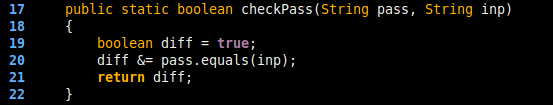
\includegraphics[width=\linewidth]{PasswordCheckerFix3}
\end{center}

Why bother going through the process of comparing strings yourself when Java provides a built-in call for
this? Lets see what jCupid thinks:

\begin{center}
  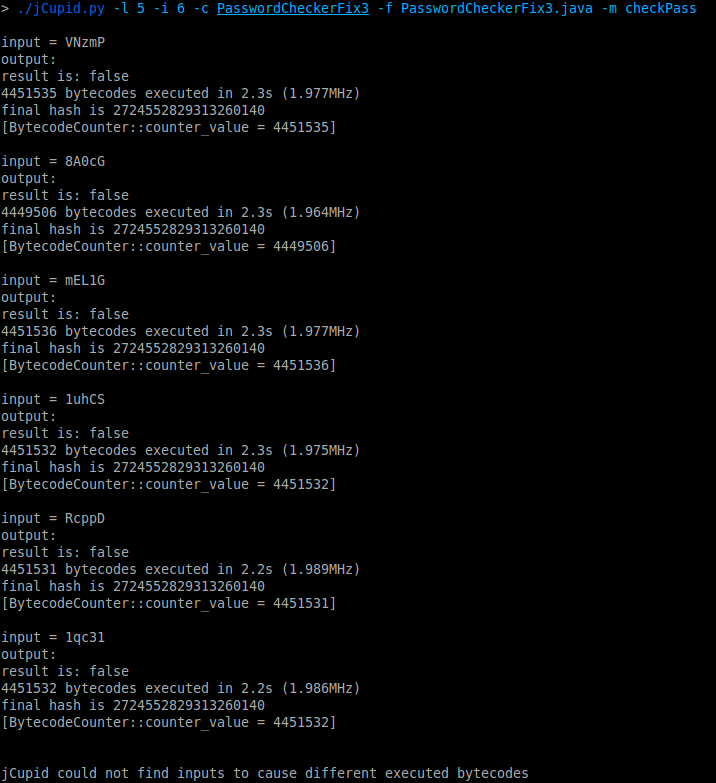
\includegraphics[width=\linewidth]{jCupidRun4}
\end{center}

It appears that all is well! jCupid doesn't notice any difference by using Java's built-in string comparison!
However after some investigation: a significant portion of Java's built-in calls are implemented in \texttt{C++}
meaning that jCupid can't detect any differences, since it only looks at the bytecodes that Java executes. And
in fact Java's built-in methods are not designed to be used in secure applications.

We provide another example: sometimes users code may not have any branches at all, but still input has an effect
on what is computed. In certain situations some inputs can cause more work to be done. In particular consider
the contrived program that reads a string from input and then sums the characters of the string to determine
how many bytes to read from a file and then hash.

Even two inputs of the same size can lead to different bytecodes being executed. So our sample program has
the following structure:

\begin{center}
  \begin{lstlisting}[language=Java]
  public class SumRandomBytes
  {
    public static void main(String [] args)
     {
       Scanner sc = new Scanner(System.in);
       String s = sc.nextLine();
      
       int sumOfBytes = sumString(s);
       byte[] data = new byte[sumOfBytes];
    
       data = readBytes(sumOfBytes);
 
       MessageDigest md = MessageDigest.getInstance(SHA-1);
       md.digest(data);
    }
 }
 \end{lstlisting}
\end{center}

jCupid catches this as:

\begin{center}
  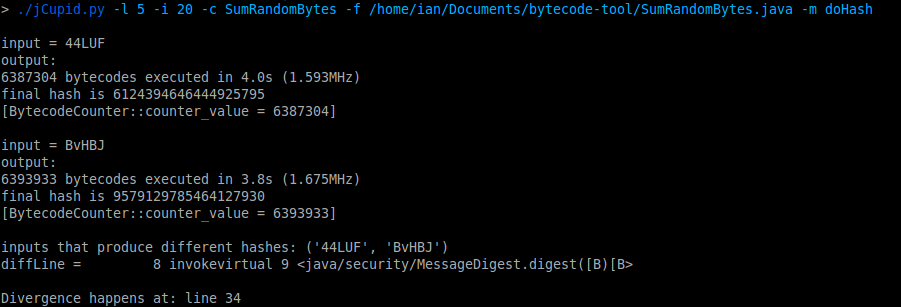
\includegraphics[width=\linewidth]{jCupidSumRandomBytes}
\end{center}

Line 34 corresponds to the \texttt{md.digest(data)} line, which tells us that something is wrong with our
hashing. Of course the issue come from the inputs: \texttt{44LUF} sums to 335 and \texttt{BvHBJ} sums to 
396, thus the first run of our program hashes 335 bytes of data where as the second run hashes 396 bytes,
which leads to a different number of bytecodes executed.


\end{document}

